\chapter{TINJAUAN PUSTAKA}
\label{chap:tinjauanpustaka}

% Ubah bagian-bagian berikut dengan isi dari tinjauan pustaka

Demi mendukung penelitian ini, dibutuhkan beberapa teori penunjang sebagai bahan acuan dan referensi. Dengan demikian penelitian ini menjadi lebih terarah.

\section{Convolutional Neural Network (CNN)}
\label{sec:cnn}

\emph{Convolutional Neural Network (CNN)} adalah salah satu jenis neural network yang biasa digunakan pada data image \cite{cit:cnn}. CNN bisa digunakan untuk mendeteksi dan mengenali object pada sebuah image. CNN adalah sebuah teknik yang terinspirasi dari cara mamalia — manusia, menghasilkan persepsi visual seperti yang terlihat pada gambar \ref{fig:kudakudaan}.

Secara garis besar Convolutional Neural Network (CNN) tidak jauh berbeda dengan neural network biasanya. CNN terdiri dari neuron yang memiliki weight, bias dan activation function. 

\begin{figure}[ht]
	\centering
	
	% Ubah dengan nama file gambar dan ukuran yang akan digunakan
	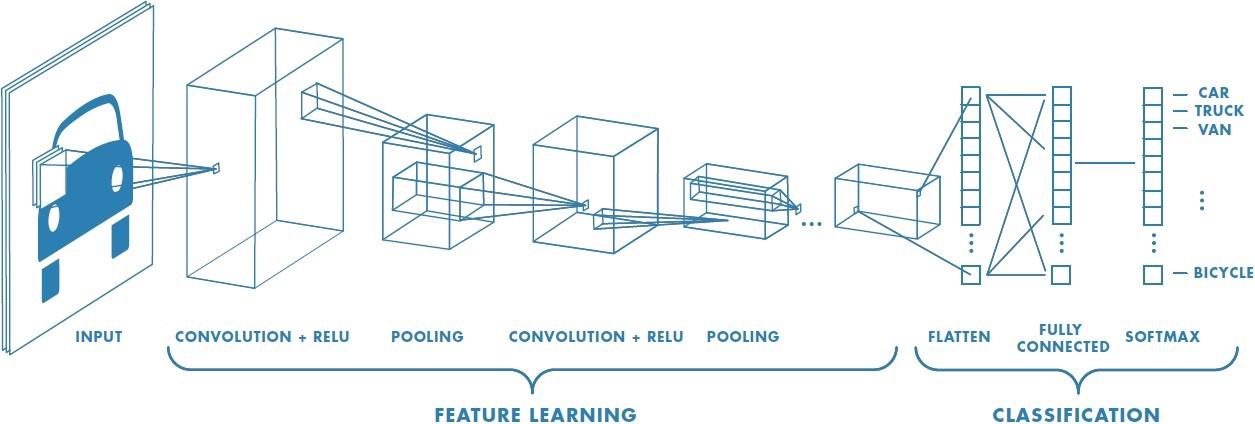
\includegraphics[width=1\columnwidth]{gambar/cnn.jpeg}
	
	% Ubah dengan keterangan gambar yang diinginkan
	\caption{Arsitektur CNN \citep{cit:cnn}}
	\label{fig:cnn}
\end{figure}

Yang membedakan CNN dari Neural network lainnya terletak pada Arsitektur dari CNN itu sendiri. Arsitektur dari CNN dibagi menjadi 2 bagian besar, \textit{\textbf{Feature Learning Layer}} dan \textit{\textbf{Classification Layer}}.

\subsection{Feature Learning}
\label{subsec:featurelearning}

Pada bagian ini CNN akan melakukan “encoding” dari sebuah image menjadi features yang berupa angka-angka yang merepresentasikan image tersebut, maka dari itu bagian ini sering juga disebut \textit{Feature Extraction Layer}. Feature Learning terdiri dari dua bagian. Convolutional Layer, Activation dan Pooling Layer.

\begin{enumerate}
	\item \textit{Convolutional Layer (Conv. Layer)}
	\begin{figure}[ht]
		\centering
		
		% Ubah dengan nama file gambar dan ukuran yang akan digunakan
		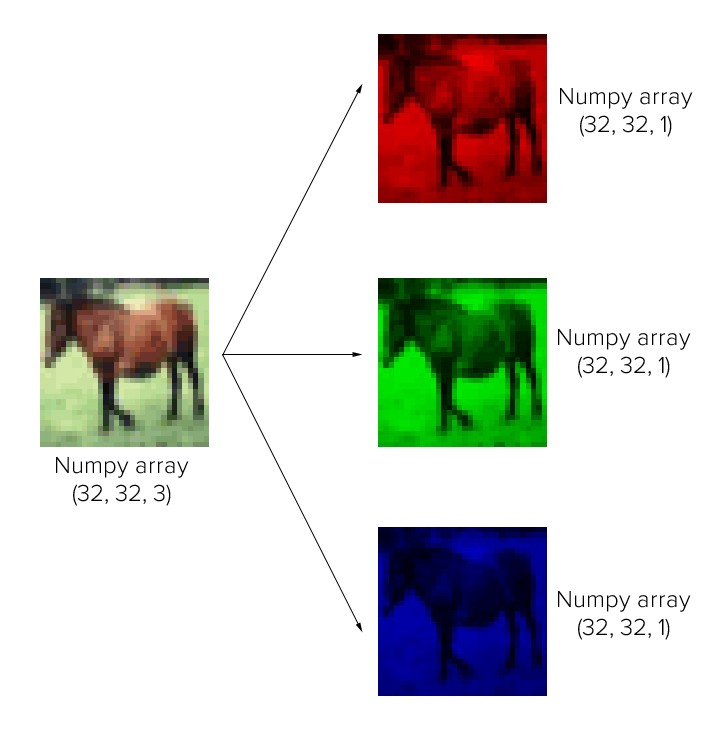
\includegraphics[width=0.7\columnwidth]{gambar/rgbhorse.jpeg}
		
		% Ubah dengan keterangan gambar yang diinginkan
		\caption{Contoh Citra RGB\citep{cit:cnn}}
		\label{fig:kudargb}
	\end{figure}
	
	Gambar \ref{fig:kudargb} adalah Citra RGB (Red, Green, Blue) berukuran 32x32 pixels yang sebenarnya adalah multidimensional array dengan ukuran 32x32x3 (3 adalah jumlah channel).
	
	Convolutional layer terdiri dari neuron yang tersusun sedemikian rupa sehingga membentuk sebuah filter dengan panjang dan tinggi (pixels). Sebagai contoh, layer pertama pada feature extraction layer biasanya adalah convolutional layer dengan ukuran 5x5x3. Panjang 5 pixels, tinggi 5 pixels dan tebal/jumlah 3 buah sesuai dengan channel dari image tersebut.
	
	Ketiga filter ini akan digeser keseluruh bagian dari gambar. Setiap pergeseran akan dilakukan operasi “dot” antara input dan nilai dari filter tersebut sehingga menghasilkan sebuah output atau biasa disebut sebagai activation map atau feature map.
	
	\begin{figure}[h]
		\centering
		
		% Ubah dengan nama file gambar dan ukuran yang akan digunakan
		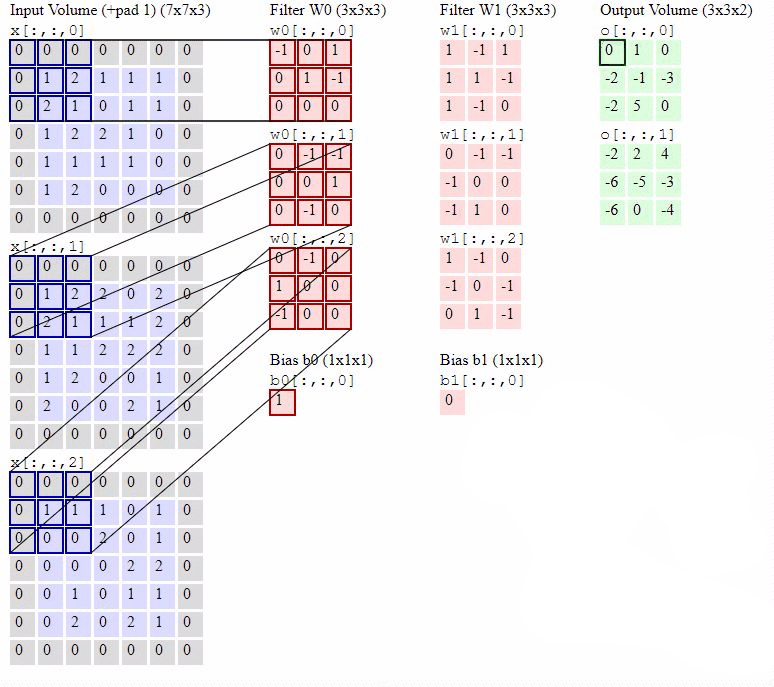
\includegraphics[width=0.9\columnwidth]{gambar/convpool.png}
		
		% Ubah dengan keterangan gambar yang diinginkan
		\caption{Convolutional Layer\citep{cit:cnn}}
		\label{fig:convolutionallayer}
	\end{figure}

	Terdapat berberapa bagian didalam Convolutional Layer, diantaranya sebagai berikut:
	
	\begin{itemize}
		\item \textit{Stride}
		
		Stride adalah parameter yang menentukan berapa jumlah pergeseran filter. Jika nilai stride adalah 1, maka conv. filter akan bergeser sebanyak 1 pixels secara horizontal lalu vertical. Pada ilustrasi diatas, stride yang digunakan adalah 2.
		
		Semakin kecil stride maka akan semakin detail informasi yang kita dapatkan dari sebuah input, namun membutuhkan komputasi yang lebih jika dibandingkan dengan stride yang besar.
		
		Namun perlu diperhatikan bahwa dengan menggunakan stride yang kecil kita tidak selalu akan mendapatkan performa yang bagus.
		
		\item \textit{Padding}
		
		Padding atau Zero Padding adalah parameter yang menentukan jumlah pixels (berisi nilai 0) yang akan ditambahkan di setiap sisi dari input. Hal ini digunakan dengan tujuan untuk memanipulasi dimensi output dari conv. layer (Feature Map).
		
		Tujuan dari penggunaan padding adalah :
		\begin{enumerate}
			\item Dimensi output dari conv. layer selalu lebih kecil dari inputnya (kecuali penggunaan 1x1 filter dengan stride 1). Output ini akan digunakan kembali sebagai input dari conv. layer selanjutnya, sehingga makin banyak informasi yang terbuang.
			
			Dengan menggunakan padding, kita dapat mengatur dimensi output agar tetap sama seperti dimensi input atau setidaknya tidak berkurang secara drastis. Sehingga kita bisa menggunakan conv. layer yang lebih dalam/deep sehingga lebih banyak features yang berhasil di-extract.
			
			\item Meningkatkan performa dari model karena conv. filter akan fokus pada informasi yang sebenarnya yaitu yang berada diantara zero padding tersebut.
		\end{enumerate}
		
		Pada ilustrasi \ref{fig:convolutionallayer}, dimensi dari input sebenarnya adalah 5x5, jika dilakukan convolution dengan filter 3x3 dan stride sebesar 2, maka akan didapatkan feature map dengan ukuran 2x2. Namun jika kita tambahkan zero padding sebanyak 1, maka feature map yang dihasilkan berukuran 3x3 (lebih banyak informasi yang dihasilkan).
		
		\newpage
		Untuk menghitung dimensi dari feature map kita bisa gunakan rumus \ref{eq:featuremap} sebagai berikut.
		
		\begin{equation}
			\label{eq:featuremap}
			output = \frac{W-N+2P}{S} + 1
		\end{equation}
		\subitem \textit{W} = Panjang/Tinggi Input
		\subitem \textit{N} = Panjang/Tinggi Filter
		\subitem \textit{P} = Zero Padding
		\subitem \textit{S} = Stride
		
	\end{itemize}

	\item \textit{Activation Layer}
	
	Setelah melalui convolution layer, nilai hasil konvolusi dikenakan fungsi aktivasi. Terdapat beberapa fungsi aktivasi yang sering digunakan pada convolutional network, di antaranya tanh() atau ReLU. Aktivasi ReLU menjadi pilihan bagi beberapa peneliti karena sifatnya yang lebih berfungsi dengan baik pada klasifikasi citra.
	
	Fungsi aktifasi ReLU adalah Fungsi maks (x,0). Jika input dari fungsi aktivasi adalah negatif maka nilai output dari neuron bisa dinyatakan sebagai 0, tapi jika nilai input dari fungsi aktivasi adalah positif maka output dari neuron adalah nilai input aktivasi itu sendiri.
	
	\item \textit{Pooling Layer}
	
	Pooling layer biasanya berada setelah conv. layer. Pada prinsipnya pooling layer terdiri dari sebuah filter dengan ukuran dan stride tertentu yang akan bergeser pada seluruh area feature map.
	
	Pooling yang biasa digunakan adalah Max Pooling dan Average Pooling. Sebagai contoh jika kita menggunakan Max Pooling 2x2 dengan stride 2, maka pada setiap pergeseran filter, nilai maximum pada area 2x2 pixel tersebut yang akan dipilih, sedangkan Average Pooling akan memilih nilai rata-ratanya.
	
	\begin{figure}[h]
		\centering
		
		% Ubah dengan nama file gambar dan ukuran yang akan digunakan
		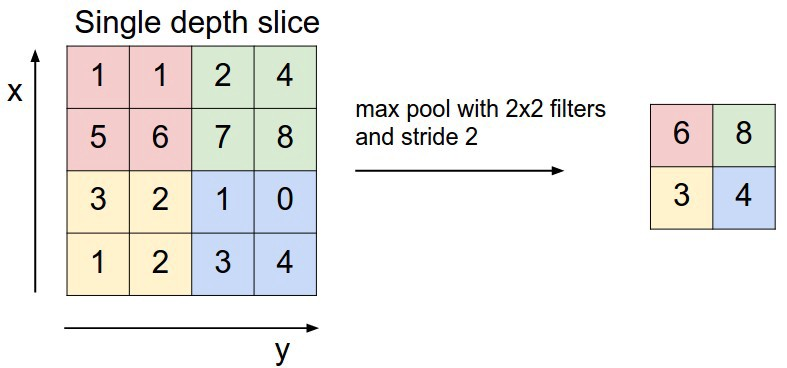
\includegraphics[width=0.7\columnwidth]{gambar/poolinglayer.jpeg}
		
		% Ubah dengan keterangan gambar yang diinginkan
		\caption{Pooling Layer\citep{cit:cnn}}
		\label{fig:poolinglayer}
	\end{figure}	
	
	Tujuan dari penggunaan pooling layer adalah mengurangi dimensi dari feature map (downsampling), sehingga mempercepat komputasi karena parameter yang harus diupdate semakin sedikit dan mengatasi overfitting.
\end{enumerate}

\vspace{2ex}
\subsection{Classification}
\label{subsec:classification}

\textit{Classification Layer} adalah bagian dari neural network yang memproses hasil dari Feature-Extraction (Feature Learning) Layer dan memberikan output berupa hasil prediksi atau klasifikasi. \textit{Classification layer} Memiliki 3 bagian Utama yaitu Flatten, Fully-Connected dan Activation.

\begin{enumerate}
	\item \textit{Flatten}
	
	Feature map yang dihasilkan dari feature extraction layer masih berbentuk multidimensional array, sehingga kita harus melakukan “flatten” atau reshape feature map menjadi sebuah vector untuk kemudian dapat diproses pada fully-connected layer.
	
	\item \textit{Fully-connected}
	
	Lapisan Fully-connected adalah lapisan dimana semua neuron aktivitas dari lapisan sebelumnya terhubung semua dengan neuron di lapisan selanjutnya seperti hal nya jaringan syaraf tiruan bisa. Setiap aktivitas dari lapisan sebelumnya perlu diubah menjadi data satu dimensi sebelum dapat dihubungkan ke semua neuron di lapisan Fully-Connected.
	
	Lapisan Fully-Connected biasanya digunakan pada metode \textit{Multi Layer Perceptron} dan bertujuan untuk mengolah data sehingga bisa diklasifikasikan. Perbedaan anatar lapisan Fully-Connected dan lapisan konvolusi biasa adalah neuron di Convolution Layer terhubung hanya ke daerah tertentu pada input. Sementara lapisan Fully-Connected memiliki neuron yang secara keseluruhan terhubung. Namun, kedua lapisan tersebut masih menggunakan operasi "dot", sehinga fungsinya tidak begitu berbeda.
	
	\item \textit{Activation}
	
	\textit{Activation layer} pada \textit{Classification} sedikit berbeda dengan yang ada pada \textit{Feature Learning} (\textit{section} \ref{subsec:featurelearning}). Fungsi yang digunakan adalah fungsi Softmax. Fungsi Softmax mengambil output dari Fully-connected layer, menggabungkannya, dan memberikan output berupa hasil klasifikasi secara keseluruhan dalam bentuk probabilitas dalam rentang nilai 0 s.d 1.
	
\end{enumerate}

\vspace{2ex}
\section{EfficientNet}
\label{sec:effnet}

\textit{EfficientNet} adalah arsitektur CNN yang dikembangkan dengan menggunakan \textit{Compound Scaling}. Tidak seperti Model \textit{Transfer Learning} pada umumnya, EfficientNet dikembangkan dengan melakukan \textit{Scaling} pada Kedalaman, Lebar, dan Resolusi model. \cite{cit:effnet}

\vspace{2ex}
\subsection{Arsitektur EfficientNet}
\label{subsec:arsitekturefn}
Varian dasar dari Model EfficientNet yaitu EfficientNet-B0 dikembangkan dari model sebelumnya sebagai model dasar. Pemilihan model dasar ini dilakukan secara otomatis menggunakan AutoML MNAS. 

\begin{figure}[h]
	\centering
	
	% Ubah dengan nama file gambar dan ukuran yang akan digunakan
	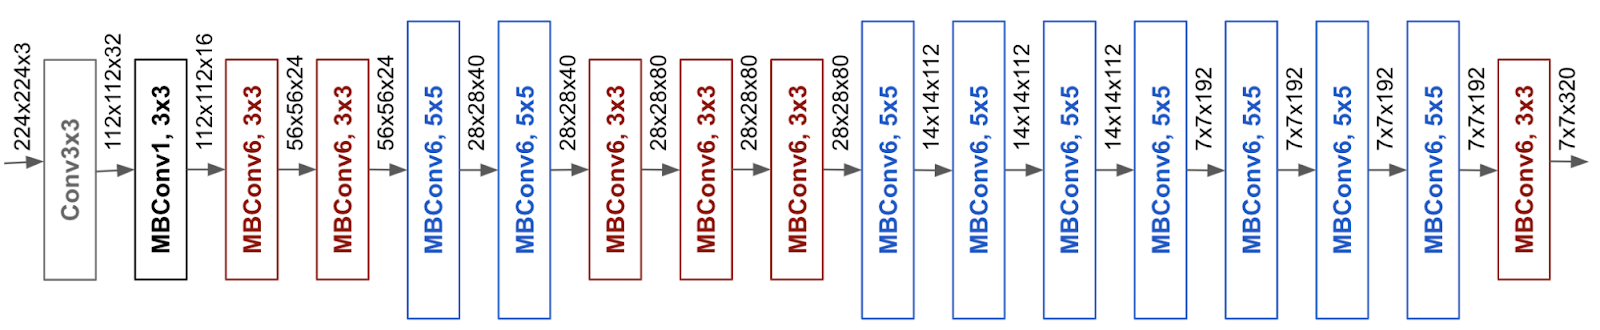
\includegraphics[width=1\columnwidth]{gambar/arsitekturefn.png}
	
	% Ubah dengan keterangan gambar yang diinginkan
	\caption{Arsitektur EfficientNet \citep{cit:effnet}}
	\label{fig:arsitektur-efn}
\end{figure}


AutoML MNAS berkerja dengan mencoba untuk mencapai akurasi tertinggi dari suatu permasalah klasifikasi (yang dalam hal ini \textit{imagenet}) dengan mencari dan menggabungkan arsitektur dari model - model yang telah ada sebelumnya secara otomatis berdasarkan skor yang mereka hasilkan melalui perbandingan Tingkat Akurasi dan Resource yang diperlukan. Dalam hal ini, model paling efisien dicapai dengan menggunakan MobileNetv2 dengan Menambahkan (squeeze-and-excitation block) ke dalamnya.

\vspace{2ex}
\subsection{Compound Scaling}
\label{subsec:compoundscaling}
\begin{figure}[h]
	\centering
	
	% Ubah dengan nama file gambar dan ukuran yang akan digunakan
	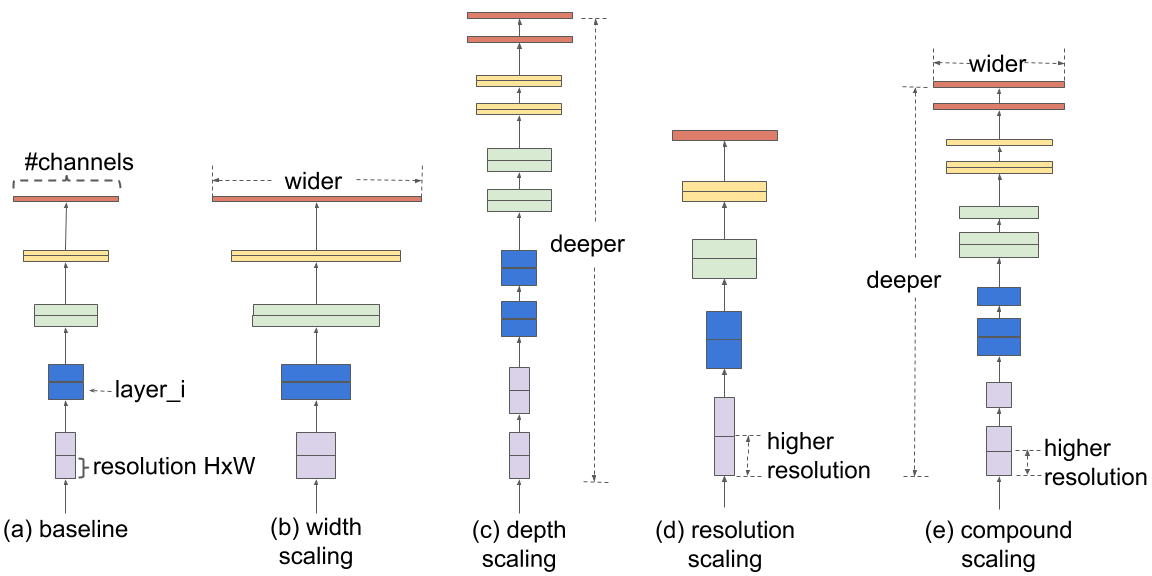
\includegraphics[width=0.9\columnwidth]{gambar/modelscaling.png}
	
	% Ubah dengan keterangan gambar yang diinginkan
	\caption{Comparison of CNN Model Scaling \citep{cit:effnet}}
	\label{fig:modelscaling}
\end{figure}

Setelah Didapat varian dasarnya (EfficientNet-B0), Compound Scaling kemudian diterapkan untuk menciptakan EfficientNet-B1 Hingga EfficientNet-B7. Dengan begitu model dengan efisien bisa didapatkan dengan menggunakan resource terbatas.

Hal ini terbukti dengan menggunakan Compound Scaling pada model sebelumnya seperti MobileNet (+1.4\% Akurasi \textit{imagenet}) dan ResNet (+0.7\% Akurasi) jika dibandingkan dengan metode scaling konvensional \cite{cit:effnet}

\vspace{2ex}
\subsection{Performa EfficientNet}
\label{subsec:efn-perf}

Pada klasifikasi dataset \textit{ImageNet} dibandingkan dengan model CNN yang telah ada sebelumnya, secara keseluruhan EfficientNet mencapai hasil akurasi dan efisiensi yang lebih baik. Bahkan, EfficientNet-B7 mencapai tingkat akurasi 84.4\% top-1 / 97.1\% top-5 pada dataset \textit{ImageNet}. ini membuat EfficientNet memiliki tingkat akurasi \textit{state-of-the-art} dari \textit{ImageNet} pada saat itu (2019)

\begin{figure}[h]
	\centering
	
	% Ubah dengan nama file gambar dan ukuran yang akan digunakan
	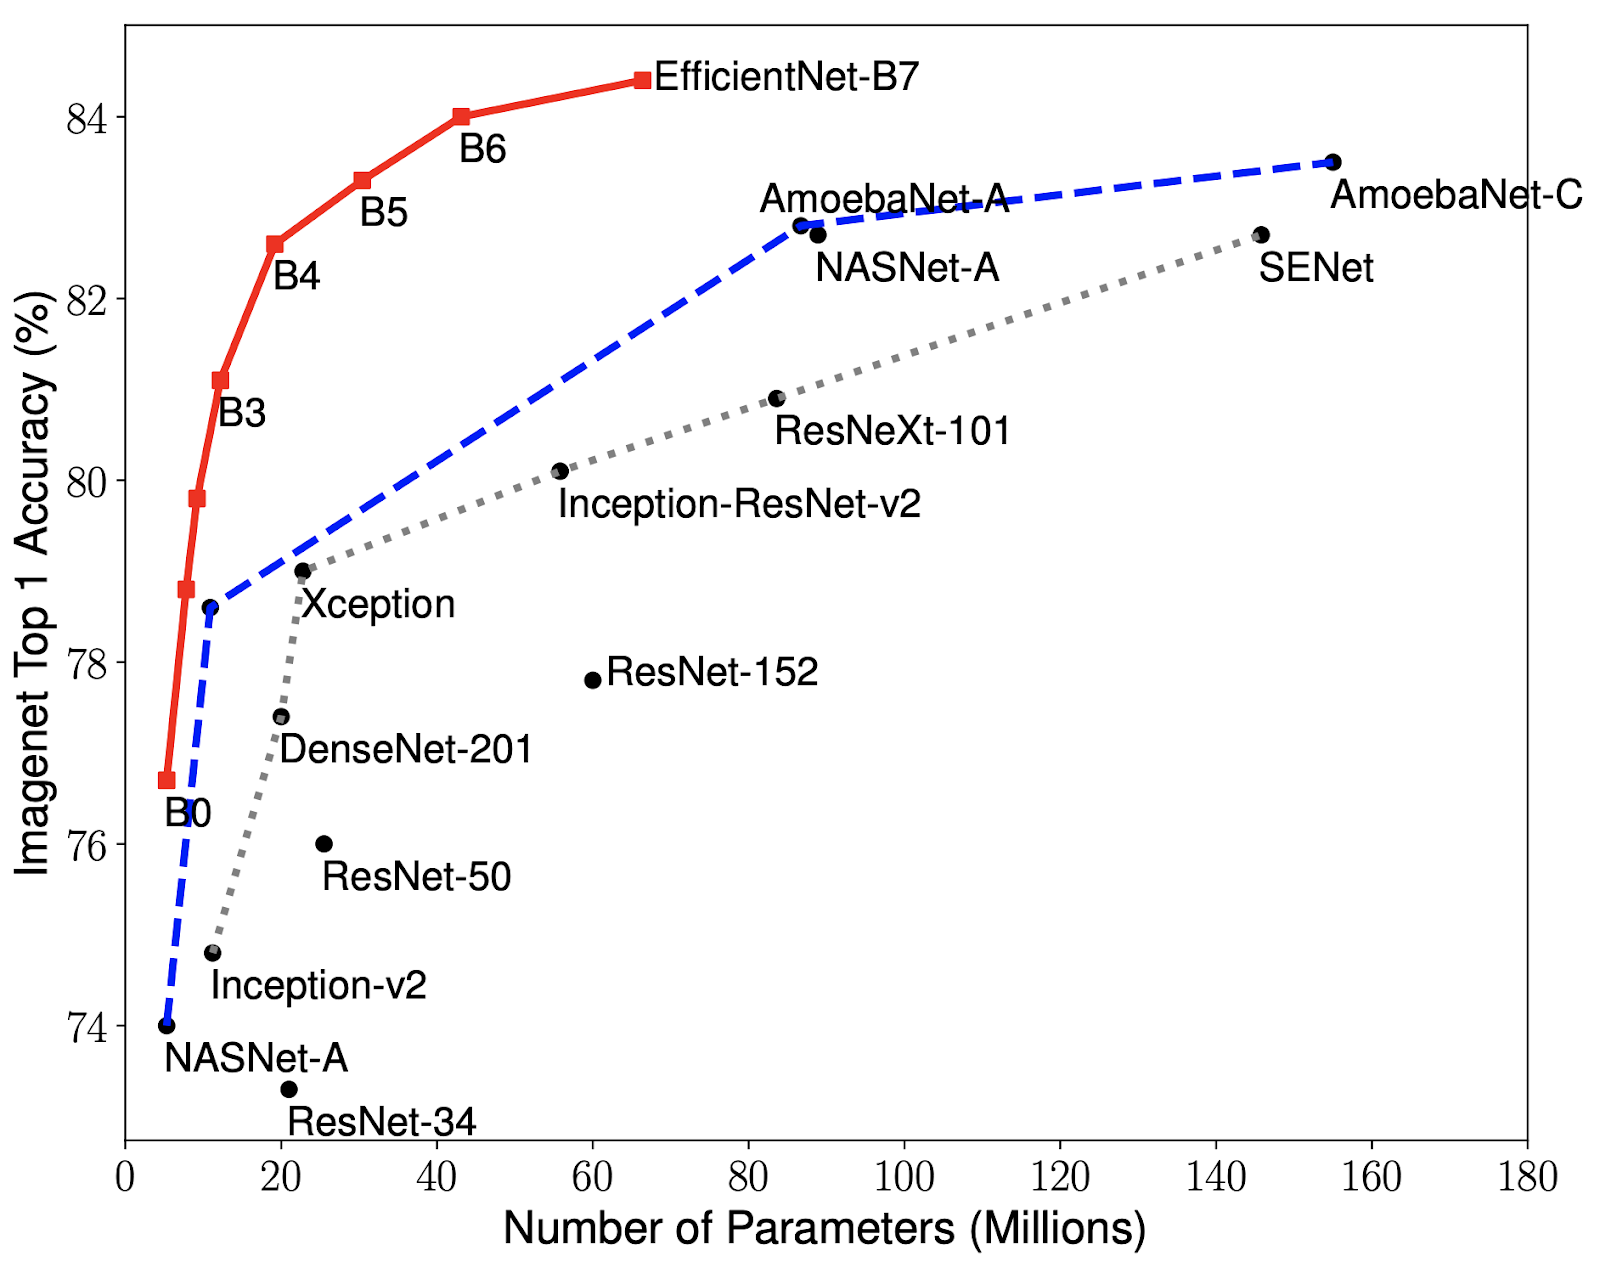
\includegraphics[width=0.9\columnwidth]{gambar/akurasiefn.png}
	
	% Ubah dengan keterangan gambar yang diinginkan
	\caption{Akurasi EfficientNet pada dataset \textit{ImageNet} \citep{cit:effnet}}
	\label{fig:akurasi-efn}
\end{figure}

EfficientNet juga diuji pada dataset lainnya dan mendapatkan akurasi \textit{state-of-the-art} pada 5 dari 8 dataset yang umum digunkan, diantaranya CIFAR-100(91.7\%) dan Flowers(98.9\%).